\section{El problema del cambio de monedas}
El problema del cambio de monedas, un desafío clásico en el campo de la optimización combinatoria y las ciencias de la computación, involucra determinar el número mínimo de monedas que se requieren para sumar una cantidad específica de dinero. Este problema se complica aún más cuando las monedas disponibles están limitadas en cantidad. La programación dinámica ofrece una metodología robusta para abordar este tipo de problemas permitiendo una solución eficiente y efectiva.

\subsection{Ejemplo 1}
Un cliente paga una cuenta de 6.20 soles con un billete de 10 soles. El cajero necesita dar el cambio con la menor cantidad de monedas posible. Las denominaciones disponibles son monedas de 1 sol, 50 céntimos, 20 céntimos y 10 céntimos con cantidades limitadas de cada una. El reto es calcular la forma óptima de entregar 3.80 soles de vuelto usando las denominaciones mencionadas. Considere que tiene 2 monedas de 1 sol, seis de 50 céntimos, cinco de 20 céntimos, y diez de 10 céntimos.

\subsubsection{Código}
\begin{lstlisting}
def min_coins_change(total, denominations, counts):
    # Convertimos las cantidades a centimos para manejarlas como enteros
    total_cents = int(total * 100)
    denominations_cents = [int(d * 100) for d in denominations]

    # Inicializamos la tabla de DP con infinito para todas las cantidades
    # excepto para 0 que necesita 0 monedas
    dp = [float('inf')] * (total_cents + 1)
    dp[0] = 0

    # Para rastrear el uso de las monedas correctamente
    used_coins = [[0 for _ in denominations] for _ in range(total_cents + 1)]

    # Procesamos cada tipo de moneda
    for i, coin in enumerate(denominations_cents):
        for j in range(coin, total_cents + 1):
            if dp[j - coin] != float('inf') and counts[i] > used_coins[j - coin][i]:
                if dp[j] > dp[j - coin] + 1:
                    dp[j] = dp[j - coin] + 1
                    used_coins[j] = used_coins[j - coin][:]
                    used_coins[j][i] += 1


    if dp[total_cents] == float('inf'):
        return "No se puede dar el cambio exacto"
    else:
        return dp[total_cents], used_coins[total_cents]

# Denominaciones de las monedas disponibles y sus cantidades
denominations = [1.0, 0.50, 0.20, 0.10]  # en soles
counts = [2, 6, 5, 10]  # cantidad de monedas disponibles

# Cantidad total a devolver
total_change = 3.80  # en soles


min_coins, coin_usage = min_coins_change(total_change, denominations, counts)

print("Numero minimo de monedas:", min_coins)
print("Uso de monedas:", coin_usage)
\end{lstlisting}

\subsubsection{Resultado}
\begin{figure}[H]
    \centering
    
\includegraphics[width=0.8\textwidth]{resultado_imagen.png}
    \caption{resultado del codigo Python.}
    \label{fig:resultado}
\end{figure}

\subsubsection{Análisis de complejidad}
\begin{figure}[H]
    \centering
    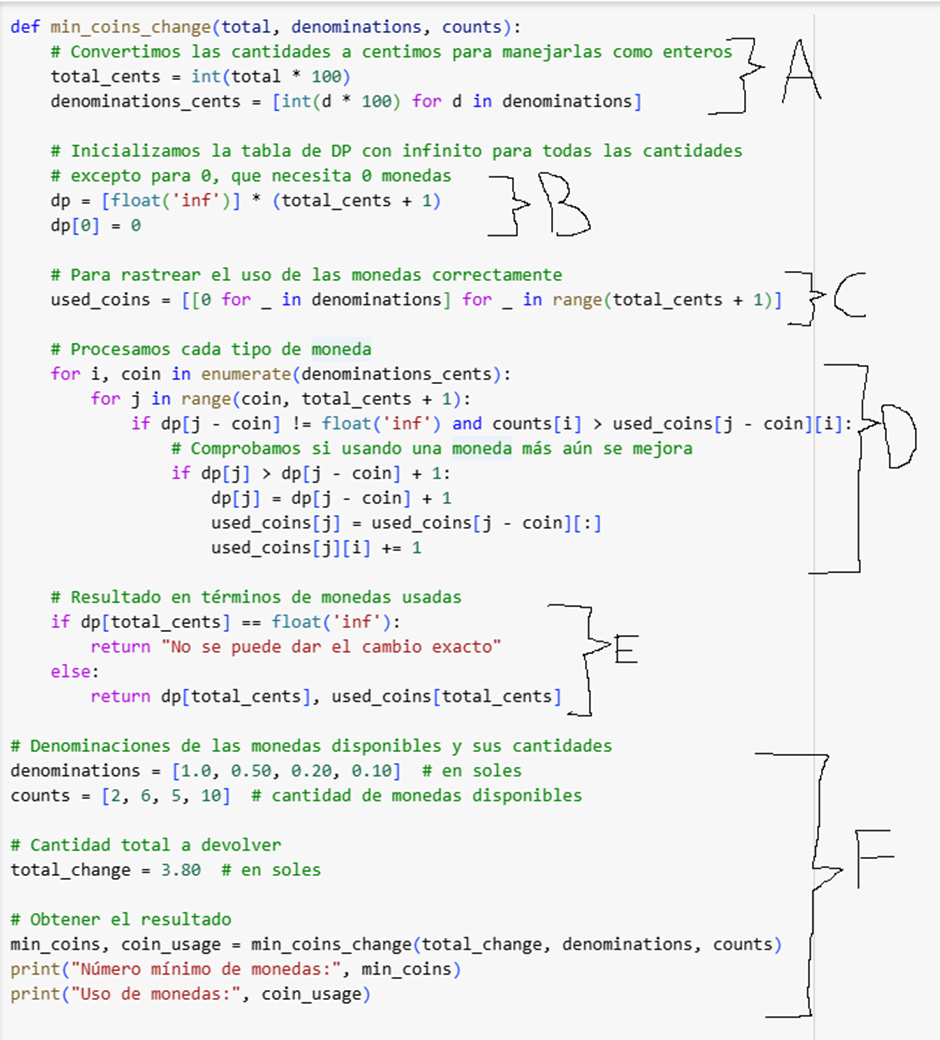
\includegraphics[width=0.8\textwidth]{complejidad_1.png}
    \caption{Analisis del codigo.}
    \label{fig:complejidad1}
\end{figure}

\begin{figure}[H]
    \centering
    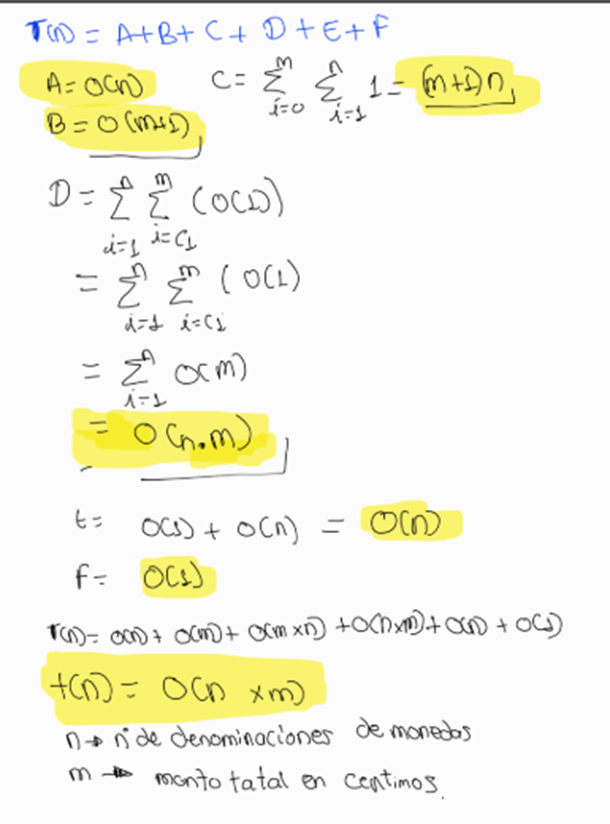
\includegraphics[width=0.8\textwidth]{complejidad_2.png}
    \caption{analisis del codigo.}
    \label{fig:complejidad2}
\end{figure}

La complejidad de este algoritmo está dada por la cantidad de denominaciones y la cantidad total a devolver, lo que resulta en una complejidad de \(O(n \cdot m)\), donde \(n\) es el número de denominaciones y \(m\) es la cantidad total a devolver.

\subsection{Ejemplo 2}
En primer lugar, debemos pensar cómo plantear el problema de forma incremental. Consideramos el tipo de moneda de mayor valor, \(X_N\). Si \(X_N > C\) entonces la descartamos y pasamos a considerar monedas de menor valor. Si \(X_N \leq C\) tenemos dos opciones: o tomar una moneda de tipo \(X_N\) y completar la cantidad restante \(C - X_N\) con otras monedas, o no tomar ninguna moneda de tipo \(X_N\) y completar la cantidad \(C\) con monedas de menor valor. De las dos opciones, nos quedamos con la que requiera un número menor de monedas. El problema lo podemos expresar de la siguiente forma cuando consideramos \(N\) tipos de monedas:

\[
Cambio(N, C) = 
\begin{cases} 
cambio(N-1, C) & \text{si } X_N > C \\
\min\{cambio(N-1, C), cambio(N, C - X_N) + 1\} & \text{si } X_N \leq C 
\end{cases}
\]

Podemos razonar análogamente para monedas de valores \(k\) menores que \(N\) y para cantidades \(C'\) menores que \(C\):

\[
Cambio(k, C') = 
\begin{cases} 
cambio(k-1, C') & \text{si } X_k > C' \\
\min\{cambio(k-1, C'), cambio(N, C' - X_k) + 1\} & \text{si } X_k \leq C' 
\end{cases}
\]

Llegamos a los casos base de la recurrencia cuando completamos la cantidad \(C\):

\[
cambio(k, 0) = 0 \quad \text{si } 0 \leq k \leq n
\]

o cuando ya no quedan más tipos de monedas por considerar, pero aún no se ha completado la cantidad \(C\):

\[
cambio(0, C') = \infty \quad \text{si } 0 < C' \leq C
\]

Podemos construir una tabla para almacenar los resultados parciales que tenga una fila para cada tipo de moneda y una columna para cada cantidad posible entre 1 y \(C\). Cada posición \(t[i,j]\) será el número mínimo de monedas necesario para dar una cantidad \(j\) con \(0 \leq j \leq C\) utilizando solo monedas de los tipos entre 1 e \(i\), con \(0 \leq i \leq n\). La solución al problema será, por tanto, el contenido de la casilla \(t[N, C]\). Para construir la tabla, empezamos rellenando los casos base \(t[i, 0] = 0\), para todo \(i\) con \(0 \leq i \leq n\). A continuación, podemos rellenar la tabla bien por filas de izquierda a derecha, o bien por columnas de arriba a abajo.

Siguiendo el método de la \textbf{programación dinámica}, se rellenará una tabla con las filas correspondientes a cada valor para las monedas y las columnas con valores desde el 1 hasta el \(N\) (12 en este caso). Cada posición \((i, j)\) de la tabla nos indica el número mínimo de monedas requeridas para devolver la cantidad \(j\) con monedas con valor menor o igual al de \(i\):

\[
\begin{array}{c|ccccccccccccc}
 & 0 & 1 & 2 & 3 & 4 & 5 & 6 & 7 & 8 & 9 & 10 & 11 & 12 \\ \hline
x = 1 & 0 & 1 & 2 & 3 & 4 & 5 & 6 & 7 & 8 & 9 & 10 & 11 & 12 \\
x = 6 & 0 & 1 & 2 & 3 & 4 & 5 & 1 & 2 & 3 & 4 & 5 & 2 & 2 \\
x = 10 & 0 & 1 & 2 & 3 & 4 & 5 & 1 & 2 & 3 & 4 & 5 & 2 & 2 \\
\end{array}
\]

En el caso anterior, hay que pagar 12 con monedas de 1, 6, 10. Supongamos que queremos pagar 12 o pagamos con 12 monedas de 1, o 2 monedas de 6, o con una de 10 y 2 de 1. Como la mejor opción es la de las monedas de 6, me quedo con esa y es la que marco en la tabla. Obsérvese que a pesar de que con monedas de 10 me haría falta 3 monedas, marco solo 2 porque es la mejor opción.

\subsubsection{Código}
\begin{lstlisting}
def min(a, b):
    return a if a < b else b

class Cambio:
    def __init__(self, cantidad, monedas):
        self.cantidad = cantidad
        self.vectorMonedas = monedas
        self.matrizCambio = self.calcularMonedas(cantidad, monedas)
        self.vectorSeleccion = self.seleccionarMonedas(cantidad, monedas, self.matrizCambio)
    
    def getVectorSeleccion(self):
        return self.vectorSeleccion
    
    def calcularMonedas(self, cantidad, monedas):
        matrizCambio = [[0 if j == 0 else 99 for j in range(cantidad + 1)] for i in range(len(monedas) + 1)]
        
        for i in range(1, len(monedas) + 1):
            for j in range(1, cantidad + 1):
                if j < monedas[i - 1]:
                    matrizCambio[i][j] = matrizCambio[i - 1][j]
                else:
                    matrizCambio[i][j] = min(matrizCambio[i - 1][j], matrizCambio[i][j - monedas[i - 1]] + 1)
        
        return matrizCambio
    
    def seleccionarMonedas(self, c, monedas, tabla):
        i, j = len(monedas), c
        seleccion = [0] * len(monedas)
        
        while j > 0:
            if i > 1 and tabla[i][j] == tabla[i - 1][j]:
                i -= 1
            else:
                seleccion[i - 1] += 1
                j -= monedas[i - 1]
        
        return seleccion

# Ejemplo de uso
cantidad = 11
monedas = [1, 5, 6, 9]

# Crear una instancia de Cambio con los valores del ejemplo
cambio_instance = Cambio(cantidad, monedas)

# Obtener el resultado de vectorSeleccion
vector_seleccion = cambio_instance.getVectorSeleccion()
print("Resultado:", vector_seleccion)
\end{lstlisting}

\subsubsection{Resultado}
Para el ejemplo dado con una cantidad de 11 y monedas de denominaciones \([1, 5, 6, 9]\), el resultado del algoritmo es el siguiente:
\begin{itemize}
    \item Utiliza 1 moneda de 5
    \item Utiliza 1 moneda de 6
    \item No utiliza monedas de 1
    \item No utiliza monedas de 9
\end{itemize}
Esto se refleja en el vector de selección: \([0, 1, 1, 0]\).

\subsubsection{Análisis de complejidad}
Inicialización de Variables y Estructuras:
\begin{itemize}
    \item \texttt{calcularMonedas(int cantidad, int[] monedas)}:
    \begin{itemize}
        \item Se inicializa una matriz de tamaño \((monedas.length + 1) \times (cantidad + 1)\).
        \item Complejidad: \(O(m \cdot n)\).
    \end{itemize}
    \item Llenado de la Matriz con Valores Iniciales:
    \begin{itemize}
        \item Complejidad: \(O(m + n)\).
    \end{itemize}
    \item Cálculo de la Matriz de Cambio:
    \begin{itemize}
        \item Complejidad: \(O(m \cdot n)\).
    \end{itemize}
    \item Selección de Monedas:
    \begin{itemize}
        \item Complejidad: \(O(m + n)\).
    \end{itemize}
    \item Función de Utilidad \texttt{min(int a, int b)}:
    \begin{itemize}
        \item Función llamada cálculo de la matriz.
        \item Complejidad: \(O(1)\) por cada llamada.
    \end{itemize}
\end{itemize}


La complejidad total del algoritmo es: \(O(m \cdot n)\). El algoritmo tiene una eficiencia polinómica en términos del número de denominaciones y la cantidad total, lo cual es razonable para muchos problemas prácticos de cambio de monedas. La matriz matrizCambio utiliza \(O(m \cdot n)\) memoria, lo cual puede ser una limitación si \(m\) o \(n\) son muy grandes.
